\section{System Implementation}

\begin{figure*}[t]
 \begin{center}
  \includegraphics[width=2\columnwidth]{figures/Fritzing_Schematics_v4.pdf}
  \caption{
    \textit{Circuit 1} consists of a temperature sensor (LM35) and a LED that turns on as the temperature rises 3\textcelsius.
    \textit{Circuit 2} has a RGB LED which changes color smoothly from aqua to green to red every increment of 3\textcelsius.
    \textit{Circuit 3} has a IC chip 74HC595 and a four-digit seven segment display  to show the temperature reading in Celsius.
    (A) and (B) are Fritzing schematics for breadboard and \papertitle, respectively. (C) shows connection arrangements hidden beneath \papertitle\ on a PCP.
  }
  \label{fig:Chosen_Circuits}
  \end{center}
\end{figure*}

% \begin{figure*}[t]
%  \begin{center}
%   \includegraphics[width=2\columnwidth]{figures/user16GesturesSV_v3.pdf}
%   \caption{ 16 heat maps display all 16 gestures performed by one of the participants. Each entry is an average heat map of 10 trials of a gesture. The sensor reading patterns are significantly different across 16 gestures.
%   }
%   \label{fig:user16GesturesSV}
%   \end{center}
% \end{figure*}

% Among the related works in the previous section, a breadboard provides easy modification by its pluggable mechanism, and PCP offers fast wiring by printing out conductive ink. Thus, we present a new rapid prototyping tool, \papertitle, simultaneously adopting a pluggable and PCP fast wiring mechanism.

Figure X shows the system flow for PCP wire routing.

\subsection{Hardware}

% Since \cite{Instant_Inkjet_Circuits} presented a successful approach to inkjet printing circuits, we adopted a similar setup with a Brother DCP-J105 printer, silver nanoparticle ink NBSIJ--MU01, resin coated paper, and transparent PET film from Mitsubishi Paper Mill.

Since \cite{Instant_Inkjet_Circuits} presented a successful approach to inkjet printing circuits, we adopted a similar setup with a Brother DCP-J105 printer and materials from Mitsubishi Paper Mill.

As illustrated in \autoref{fig:figure1}a, \papertitle\ possesses a multi-layer design composed of customized PCBs. The top layer consists of 10-by-30 female headers resembling the appearance and the pluggable mechanism of a breadboard. \autoref{fig:figure1}d indicates the bottom layers where pieces of PCP are placed. The wiring on each piece of PCP determines the connections for the component pins on the top layer. 
% Despite showing only X layers in Figure X, \papertitle\ can stack up to even more layers to create more connections which support more complicated circuits.

Each pin and contact pad in zone A on both the top layer and the bottom layers connects to its corresponding pad on zone B (\autoref{fig:figure1}e). Each pad in zone B then contacts and electrically connects to its neighboring layers through a compressible on-board contact spring (\autoref{fig:figure1}c and \autoref{fig:figure1}f). Pads in zone A on the bottom layers are also equipped with the same contact spring to push against the conductive ink on a PCP to form reliable physical contacts. Lastly, the layers and pieces of PCP are assembled and stacked up through tightening four screws on 4 corners.

However, tightening the four screws on the corners causes the PCB to flex outwards by approximately 1 mm. The compression range of a contact spring is only 0.5 mm; therefore, additional forces must be exerted in order to mitigate the outward flex and ensure the reliability for electrical connection. We successfully used acrylic backboards to evenly distribute the force across the PCB and minimize flex (\autoref{fig:figure1}b). Using a piece of PCP that allows for electrical conductivity throughout all points, we tested any two points on \papertitle\ to find successful conductivity for all test cases. Future hardware designers should evenly distribute the force across the entire board via an additional rigid support structure such as acrylic. Other options include exchanging the current contact springs for those with greater compression range.

Because of the aforementioned bottom layer structure, vertical expansion is not limited to only  layers despite showing only 2 bottom layers in \autoref{fig:figure1}a. Stacking multiple bottom layers still maintain electrical conductivity, and at the same time creates more connections, leading to complicated circuits being supported and solving the issue of PCP's flaw of only able to span one layer.

\subsection{Modification} %System flow?
% Figure X shows the system flow for PCP wire routing.
When an error occurs and wiring needs to be fixed, users do not need to perform any changes to the placed components. Instead, users modify the wiring of the PCP in the GUI, re-export and print out the modified PCP. Then, users swap out the non-working PCP to conclude the modification process.

% To create wire routing on PCP for \papertitle, the Breadboard Tab in Fritzing \cite{Fritzing} functions as an interface (Figure X) for users to place components and arrange connections on a custom part, \papertitle. Then, the connection information saved in a Fritzing file, extracted through a Python script, is exported to a PCB design software, EAGLE \cite{EAGLE} where final connection arrangements and autorouting for PCP are created via EAGLE user language programming (ULP) scripts.

% \begin{figure}
%   \begin{center}
%   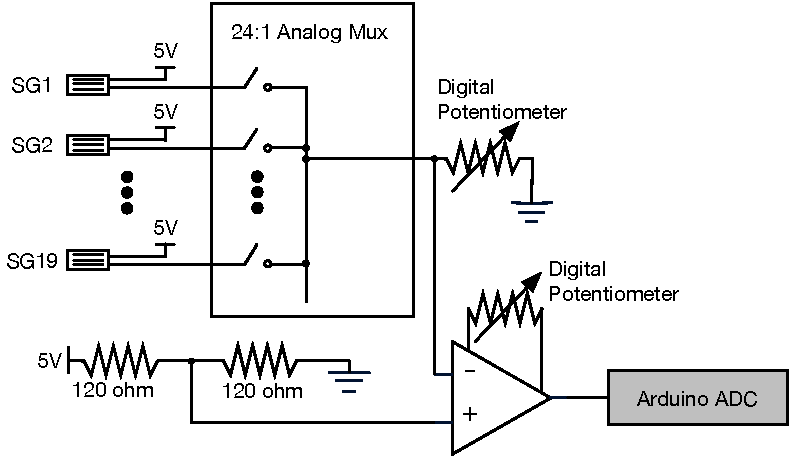
\includegraphics[width=1\columnwidth]{figures/Implementation.pdf}
%   \caption{The mechinical design of \papertitle }
%   \label{fig:FIGURE2}
%   \end{center}
% \end{figure}


% \begin{figure}
%   \begin{center}
%   \includegraphics[width=1\columnwidth]{figures/GUI.png}
%   \caption{\papertitle also provides users a graphic user interface to help them design circuits efficiently.}
%   \label{fig:FIGURE4}
%   \end{center}
% \end{figure}